% Copyright 2016 - 2017 Bas van Meerten and Wouter Franssen
%
%This file is part of ssNake.
%
%ssNake is free software: you can redistribute it and/or modify
%it under the terms of the GNU General Public License as published by
%the Free Software Foundation, either version 3 of the License, or
%(at your option) any later version.
%
%ssNake is distributed in the hope that it will be useful,
%but WITHOUT ANY WARRANTY; without even the implied warranty of
%MERCHANTABILITY or FITNESS FOR A PARTICULAR PURPOSE.  See the
%GNU General Public License for more details.
%
%You should have received a copy of the GNU General Public License
%along with ssNake. If not, see <http://www.gnu.org/licenses/>.

\documentclass[11pt,a4paper]{article}
% Copyright 2016 - 2017 Bas van Meerten and Wouter Franssen
%
%This file is part of ssNake.
%
%ssNake is free software: you can redistribute it and/or modify
%it under the terms of the GNU General Public License as published by
%the Free Software Foundation, either version 3 of the License, or
%(at your option) any later version.
%
%ssNake is distributed in the hope that it will be useful,
%but WITHOUT ANY WARRANTY; without even the implied warranty of
%MERCHANTABILITY or FITNESS FOR A PARTICULAR PURPOSE.  See the
%GNU General Public License for more details.
%
%You should have received a copy of the GNU General Public License
%along with ssNake. If not, see <http://www.gnu.org/licenses/>.

\usepackage[british]{babel}
\usepackage{graphicx,booktabs,listings,amsmath,pgfplots,pgfplotstable}
\usepackage[small,bf,nooneline]{caption}
\usepackage{subcaption}
\usepackage[sort&compress,numbers]{natbib}
\usepackage{tikz}
\usepackage{mathtools}
\usepackage[nottoc]{tocbibind}%adds bibliography to table of contents.
\graphicspath{{./images/}}
%\setlength{\textwidth}{453pt} %597 pt is the a4 paperwidth. Minus 2 in margin. 72 pt = 1 in
%\setlength{\hoffset}{-\oddsidemargin}
%\setlength{\voffset}{-30pt} %
%\setlength{\textheight}{651 pt} %a4 height 845 pt minus 2* total headheight. In this case 2*88pt
%% examine margines via the layout package. Use command \layout{} in document to draw a picture.
%\setlength{\parindent}{0.5 cm}
%\setlength{\parskip}{0 cm}
\usepackage[left=82pt,right=82pt,top=95pt,bottom=95pt,footnotesep=0.5cm]{geometry}
%\setlength{\headheight}{14pt}

%define colours--------------------
%dark
\usepackage{xcolor}
\definecolor{MyGrayD}{RGB}{1,1,1}
\definecolor{MyRedD}{RGB}{237,45,46}
\definecolor{MyGreenD}{RGB}{0,140,71}
\definecolor{MyBlueD}{RGB}{24,89,169}
\definecolor{MyOrangeD}{RGB}{243,125,34}
\definecolor{MyPurpleD}{RGB}{102,44,145}
\definecolor{MyBrownD}{RGB}{161,29,32}
\definecolor{MyPinkD}{RGB}{179,56,147}
%normal
\definecolor{MyGray}{RGB}{114,114,114}
\definecolor{MyRed}{RGB}{241,89,95}
\definecolor{MyGreen}{RGB}{121,195,106}
\definecolor{MyBlue}{RGB}{89,154,211}
\definecolor{MyOrange}{RGB}{249,166,90}
\definecolor{MyPurple}{RGB}{158,102,171}
\definecolor{MyBrown}{RGB}{205,112,88}
\definecolor{MyPink}{RGB}{215,127,179}
%light
\definecolor{MyGrayL}{RGB}{204,204,204}
\definecolor{MyRedL}{RGB}{242,174,172}
\definecolor{MyGreenL}{RGB}{216,228,170}
\definecolor{MyBlueL}{RGB}{184,210,235}
\definecolor{MyOrangeL}{RGB}{242,209,176}
\definecolor{MyPurpleL}{RGB}{212,178,211}
\definecolor{MyBrownL}{RGB}{221,184,169}
\definecolor{MyPinkL}{RGB}{235,191,217}
%----------------------------------

%Figure ref with hyperref
\newcommand{\fref}[1]{\hyperref[#1]{Figure \ref*{#1}}}
\newcommand{\sref}[1]{\hyperref[#1]{Section \ref*{#1}}}
\newcommand{\tref}[1]{\hyperref[#1]{Table \ref*{#1}}}

%Makes a new command for figures with input values: filename, width(times linewidth),
% caption and label.
\newcommand{\onefigure}[4]{
\setlength{\captionwidth}{#2\linewidth}
\begin{figure}
\includegraphics[width=#2\linewidth]{#1}
\centering
\parbox{\linewidth}{\caption{#3}
\label{#4}}
\end{figure}
}

%Makes a new command for tikz figures with input values: tikz commands, 
% caption and label.
\newcommand{\onetikz}[3]{
\settowidth{\captionwidth}{#1}
\ifthenelse{\lengthtest{\captionwidth<0.7\linewidth}}{\setlength{\captionwidth}{0.7\linewidth}}{}

\begin{figure}
\centering
#1
\centering
\parbox{\linewidth}{\caption{#2}
\label{#3}}
\end{figure}
}

%Makes a new command for two figures next to each other with input values: filename1, caption1, label1,filename2, caption2 and label2. Figure width is set to 0.47\linewidth and the space between the figures is filled with \hfill so the sides of the figures align with to edge of the line.
\newcommand{\twofigure}[6]{
\setlength{\captionwidth}{\linewidth}
\begin{figure*}[ht!]
\begin{minipage}[t]{0.47\linewidth}
\includegraphics[width=\linewidth]{#1}
\centering
\caption{#2}
\label{#3}
\end{minipage}
\hfill
\begin{minipage}[t]{0.47\linewidth}
\centering
\includegraphics[width= \linewidth]{#4}
\centering
\caption{#5}
\label{#6}
\end{minipage}
\end{figure*}
}


%Makes a new command for a table with caption witdh equal to the total table width. Input: tabular, caption and label. Example:
%\onetable{
%\begin{tabular}{ccc}
%a&b&c\\
%\hline
%1&1&1\\
%1&1&1\\
%1&1&1\\
%\end{tabular}
%{The caption.}
%{tab:table1}
%}
\newcommand{\onetable}[3]{
\settowidth{\captionwidth}{#1}
\ifthenelse{\lengthtest{\captionwidth<0.7\linewidth}}{\setlength{\captionwidth}{0.7\linewidth}}{}
\begin{table}
\caption{#2}
\vspace{-0.24cm} %Puts caption close to toprule
\label{#3}
\centering
#1
\end{table}
}

%Makes a long table with captionwidth equal to tablewidth. It takes the following arguments:
%1: Column specifier (e.g. cccc)
%2: Caption
%3: Label
%4: First head (i.e. first row of regular table)
%5: Head of consecutive pages
%6: Foot of pagebreak
%7: Lastfoot (e.g. \midrule)
%8: Body of table
\newcommand{\onelongtable}[8]{
\begin{center}
\settowidth{\captionwidth}{
\begin{tabular}{#1}
#4
#8
\end{tabular}} % This ends the captionwidth part. Next comes the real table.

\begin{longtable}{#1}
\caption{#2}\\
\vspace{-0.74cm} %Puts caption close to toprule
\label{#3}\\

#4
\endfirsthead

#5
\endhead

#6
\endfoot

#7
\endlastfoot

#8
\end{longtable}
\end{center}}




%1:pgfplots code
%2:width
%3:caption
%4:label
\newcommand{\pgfplotsfigure}[4]{
\pgfplotsset{width=#2\linewidth}
\setlength{\captionwidth}{#2\linewidth}
\begin{figure}[t]
\centering
#1
\centering
\parbox{\linewidth}{\caption{#3}
\label{#4}}
\end{figure}
}


\usepackage[bitstream-charter]{mathdesign}
\usepackage[T1]{fontenc}
\usepackage[protrusion=true,expansion,tracking=true]{microtype}
\pgfplotsset{compat=1.7,/pgf/number format/1000 sep={}, axis lines*=left,axis line style={gray},every outer x axis line/.append style={-stealth'},every outer y axis line/.append style={-stealth'},tick label style={font=\small},label style={font=\small},legend style={font=\footnotesize}}
\usepackage{colortbl}
\usetikzlibrary{calc}

%Set section font
\usepackage{sectsty}
\allsectionsfont{\color{black!70}\fontfamily{SourceSansPro-LF}\selectfont}
%--------------------


%Set toc fonts
\usepackage{tocloft}
%\renewcommand\cftchapfont{\fontfamily{SourceSansPro-LF}\bfseries}
\renewcommand\cfttoctitlefont{\color{black!70}\Huge\fontfamily{SourceSansPro-LF}\bfseries}
\renewcommand\cftsecfont{\fontfamily{SourceSansPro-LF}\selectfont}
%\renewcommand\cftchappagefont{\fontfamily{SourceSansPro-LF}\bfseries}
\renewcommand\cftsecpagefont{\fontfamily{SourceSansPro-LF}\selectfont}
\renewcommand\cftsubsecfont{\fontfamily{SourceSansPro-LF}\selectfont}
\renewcommand\cftsubsecpagefont{\fontfamily{SourceSansPro-LF}\selectfont}
%--------------------

%Define header/foot
\usepackage{fancyhdr}
\pagestyle{fancy}
\fancyhead[LE,RO]{\fontfamily{SourceSansPro-LF}\selectfont \thepage}
\fancyhead[LO,RE]{\fontfamily{SourceSansPro-LF}\selectfont \leftmark}
\fancyfoot[C]{}
%--------------------

%remove page number from first chapter page
\makeatletter
\let\ps@plain\ps@empty
\makeatother
%----------------------
\usepackage{blindtext, color}
\definecolor{gray75}{gray}{0.75}
\newcommand{\hsp}{\hspace{20pt}}



\usepackage[hidelinks,colorlinks,allcolors=black, pdftitle={VOCS},pdfauthor={W.M.J.\ Franssen}]{hyperref}

\interfootnotelinepenalty=10000 %prevents splitting of footnote over multiple pages
\linespread{1.2}

%\usepgfplotslibrary{external}%creates all external tikz images that are included.
%\tikzexternalize[shell escape=-enable-write18]%activate externalization
%\tikzsetexternalprefix{GeneratedFigures/}
%\tikzset{external/force remake} %Enable forced remake

\title{\color{black}\fontfamily{SourceSansPro-LF}\bfseries Variable Offset Cumulative Spectra (VOCS)
analysis in ssNake}
\author{}
\date{\color{black}\fontfamily{SourceSansPro-LF}\bfseries \today}


\begin{document}
%\newgeometry{left=72pt,right=72pt,top=95pt,bottom=95pt,footnotesep=0.5cm}
\microtypesetup{protrusion=true} % enables protrusion

\maketitle

\section{Introduction}
This tutorial will explain how a VOCS (Variable Offset Cumulative Spectra) experiment can be processed using ssNake.
The tutorial provided with the ssNake program is considered as prior knowledge.
If you have not yet studied this, please do so before continuing with this example.

When encountering very broad signals in solid state NMR, issues arise with proper excitation and acquisition. As the broad signal decays very fast in the time domain (FID), an echo is required to properly detect it.
The width of the spectrum that can be covered by these echo pulse is however limited by the RF power.
In cases with extremely broad signals, a regular probe cannot reach RF powers high enough to excite the entire spectrum at once.

To counter this problem, the VOCS experiment has been developed.
The idea is simple: echo spectra are recorded for several different offsets (carrier frequencies) and added afterwards.
While each experiment only excites a relatively small part, the entire spectrum can be reconstructed as long as we obtain several echo spectra with offset values across the broad line.
Processing the data can be a bit cumbersome, but its principles are easy.

\section{Used data}
For this example, we will use a set of $^{127}$I spectra of methylammonium iodide (MAI) recorded at 20~T.
21 echos were recorded with 100 kHz steps in the offset (carrier frequency).
The spectrum is very broad due to the strong quadrupolar coupling.
The lineshape is only of the central transition, and is dominated by the second order quadrupolar coupling.

In the data directory, 21 different spectra are saved as MATLAB files (saved with ssNake).
The 'Raw' folder contains the acquired FID from the Varian spectrometer.
The `FinalSpectrum' folder contains the final spectrum of this tutorial.

\section{Processing}
In the data directory, 21 different spectra are saved as MATLAB files. The saved spectra contain the
processed echo spectra. These have been made using whole echo processing (see our other tutorial).
The center frequencies has been put right (necessary because I recorded the data as an array,
instead of the better option to take spectra 1D spectra), and the data have been cut to only show
the relevant area (we do not want to add all the noise to the left and right of every echo).

\begin{itemize}
\item Open the data in ssNake by dragging and dropping all of them in ssNake (or via File $\longrightarrow$ Open).
\end{itemize}
This will open all the separate echoes in different workspaces.
To preview the data, lets view them together in a Multiplot.
When in the spectrum called '-100', use Plot $\longrightarrow$ Multiplot to open the multiplot window.
Use the `Add spectrum' button in the side frame to add some other echos, and reset the spectrum view by double right click in the spectrum.
When the -1000, -700, -400, 200, and 600 spectra are added, the view should look similar to:

\begin{center}
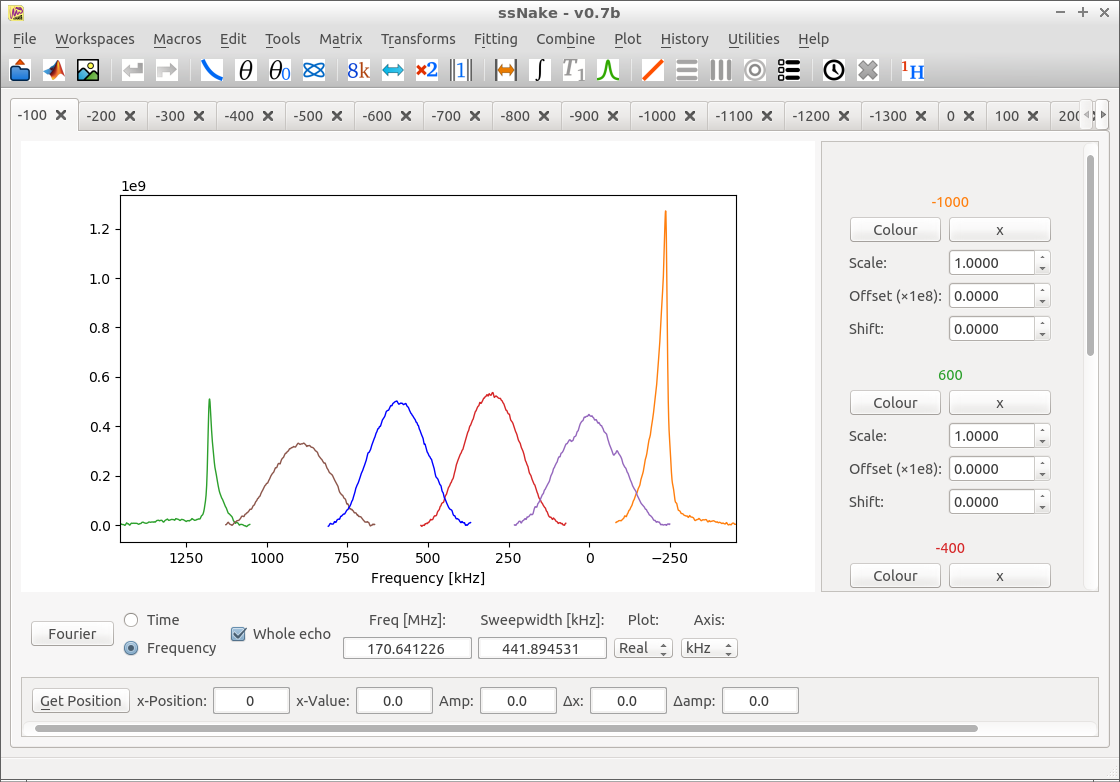
\includegraphics[width=0.8\linewidth]{Figs/Fig1.png}
\end{center}

We can already see a hint of what the entire spectrum will look like (spoiler alert: it has $\eta=0$).

The actual tricky part is adding the data together: each echo has its own $x$-axis, and we can not just add the data.
We first should force all the spectra to use the same $x$-axis.
This is called `regridding'.
In a regridding procedure, interpolation is used to obtain the data points along a new $x$-axis.
All the new $x$-values that are outside the range of the old axis will have $y$-values of 0 (no \textit{extra}polation is performed).

We need to apply the same regridding on all of our 21 spectra.
Based on the figure above, a range of $-500$ to 1500 kHz seems appropriate.
We also have to chose a total number of points.
It is good to use about the same density (number of points per kHz) as our single echoes.
This appear to be about 1.6 point per kHz, so lets make it 2 and go for 4k points (4096 points). 


\begin{itemize}
\item Go to workspace `-100' 
 \item Execute Matrix $\longrightarrow$ Regrid (min: -500, max: 1500, points 4096).
\end{itemize}

This should result in the following Figure:

\begin{center}
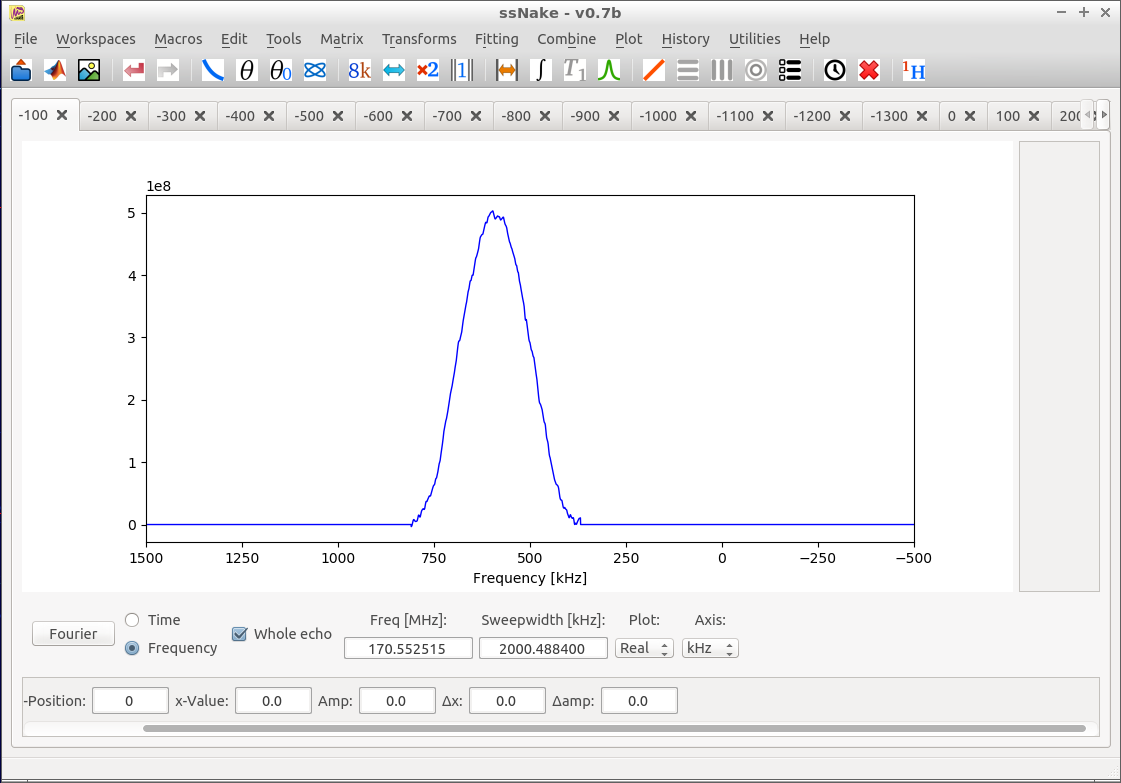
\includegraphics[width=0.8\linewidth]{Figs/Fig2.png}
\end{center}
We now have to perform this for all the workspaces.
This is most easily done by using a macro.
Go to workspace `-200' and go to Menu Macros $\longrightarrow$ Start recording and push OK for the name.
Then perform the same regridding as before (min: -500, max: 1500, points 4096).
Then go to Macros $\longrightarrow$ Stop recording.
The macro can now be used via Macros $\longrightarrow$ Run $\longrightarrow$ MacroName.
Run the macro over all the other workspaces to perform the regridding for all 21 spectra.

As a final step, we have to add all the spectra.
This can be most conveniently done by merging the data to a 2D data set.
Use Combine $\longrightarrow$ Combine Workspaces and select all entries on the left (use ctrl + a), and drag them to the right.
Push OK, and give a name to the new workspace.
This creates a 2D data set, with the spectra along D1.
To view this, use Plot $\longrightarrow$ Stack plot, and set the `Spacing' to zero (in the side frame).
This looks like this:

\begin{center}
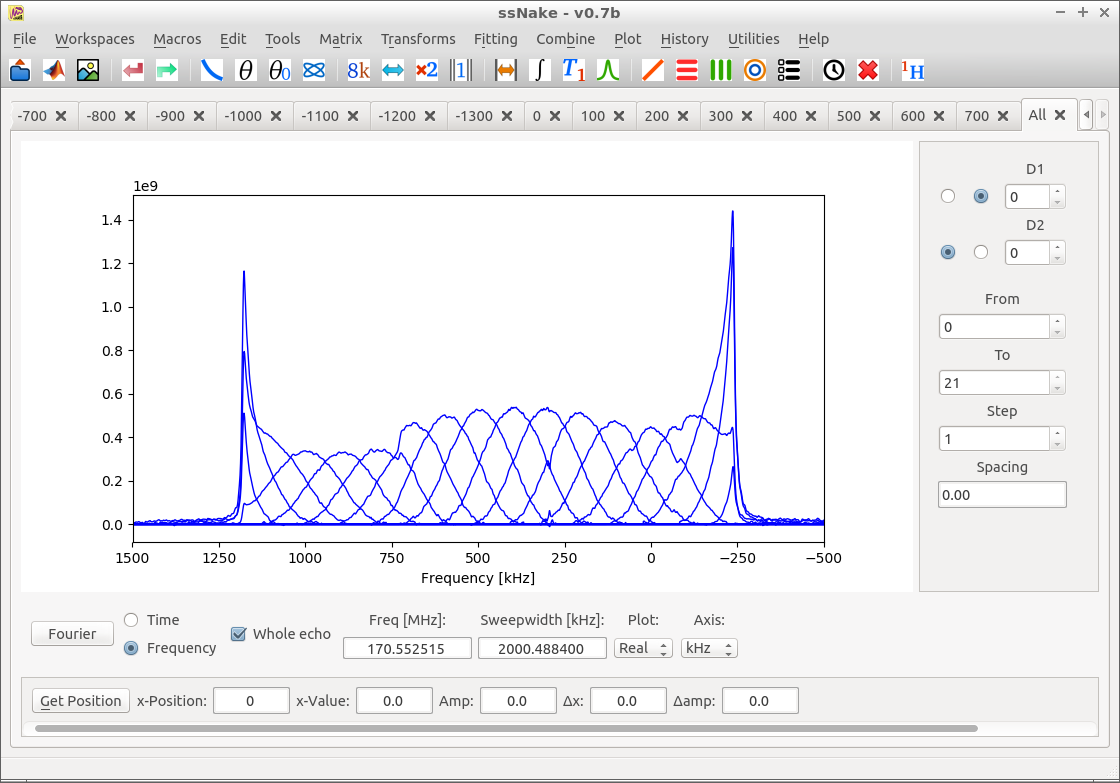
\includegraphics[width=0.8\linewidth]{Figs/Fig3.png}
\end{center}

Which shows all the different spectra overlaid.
As a final step, we need to sum the data along D1:
\begin{itemize}
\item Go to a 1D plot (Plot $\longrightarrow$ 1D Plot)
\item Change the active dimension to D1 (click on the radio button under `D1' in the side frame)
\item Use Matrix $\longrightarrow$ Region $\longrightarrow$ Sum (with no input parameters, just press Ok)
\end{itemize}
This should result in:
\begin{center}
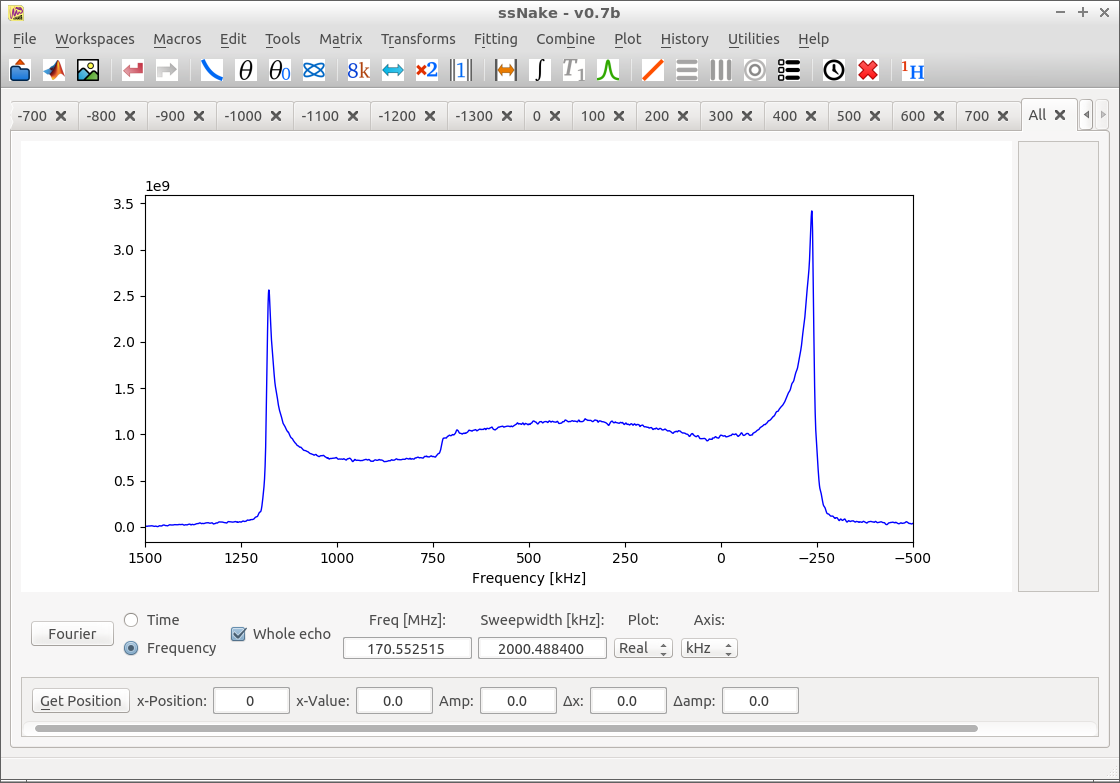
\includegraphics[width=0.8\linewidth]{Figs/Fig4.png}
\end{center}
Which is the final spectrum.
A beautiful $\eta = 0$ second order quadrupolar pattern.
It does not exactly match with simulations, as the probe tuning was not changed during the experiment.
This lowers the intensity far away from the centre.
Also, the `step' in the centre is not at the correct position.
This is probably due to some chemical shift anisotropy (CSA).


\end{document}
